% chapters/02_analysis.tex
\chapter{比赛题目分析和相关资料调研}

\section*{本章调研发现速览}

\begin{table}[H]
    \centering
    \begin{tabular}{p{0.20\textwidth}p{0.35\textwidth}p{0.35\textwidth}}
        \toprule
        \textbf{调研方向} & \textbf{核心发现} & \textbf{对本项目的启示} \\
        \midrule
        Linux Device Mapper & dm-crypt 使用 XTS-AES + plain64 IV；dm-verity 使用 SHA-256 Merkle 树 + on-disk 哈希树布局 & 必须与 Linux 逐字节兼容，否则无法与 cryptsetup 互操作 \\
        Asterinas 内核架构 & Framekernel + OSTD + BIO 异步 I/O + \texttt{no\_std} 环境 & 无法复用 Linux 代码，需从头设计 Rust 实现，适配 BIO 路径 \\
        AES-XTS 标准 & NIST SP 800-38E 定义 XTS-AES；Linux 使用 AES-256-XTS 双密钥 & 需严格遵循标准，并通过固定向量验证兼容性 \\
        SHA-256 标准 & FIPS 180-4 定义；Linux dm-verity 使用 32 字节摘要 & 需实现纯 Rust SHA-256，无外部依赖 \\
        Rust 系统编程 & 所有权、借用检查、trait 系统、\texttt{no\_std} 支持 & 可构建内存安全的存储框架，类型系统可编码安全能力 \\
        \bottomrule
    \end{tabular}
\end{table}

\section{比赛题目分析}

\subsection{赛题背景与核心要求}

全国大学生计算机系统能力大赛操作系统设计赛功能挑战赛道要求参赛队在星绽操作系统（Asterinas）上使用 Rust 编程语言实现 \texttt{dm-crypt} 与 \texttt{dm-verity} 功能。赛题明确提出了五项技术指标：

\begin{enumerate}
    \item \texttt{dm-verity} 基础功能：构建 SHA-256 哈希树，实现数据块完整性验证，支持内核启动参数配置；
    \item \texttt{dm-crypt} 基础功能：透明加解密 I/O 路径，作为后端支撑 \texttt{cryptsetup} 对加密卷的创建和管理；
    \item 根文件系统加密：使用 \texttt{dm-crypt} 加解密根文件系统；
    \item 性能与启动要求：I/O 吞吐及延迟接近 Linux，\texttt{dm-verity} 不显著增加内核启动时间；
    \item 技术探索：探索基于 Rust OS 的可信存储性能优化技术。
\end{enumerate}

这些要求覆盖了功能完整性、Linux 兼容性、性能可观测性和技术创新性四个维度。本项目在全部五个指标上均已完成并通过验证。

星绽操作系统采用 Framekernel 架构，通过 OSTD 框架将内核核心组件运行于非特权级，实现了可信计算基（TCB）的最小化。这一架构在提供强安全保障的同时，也意味着星绽的内核接口（BIO 系统、设备注册、启动流程）与 Linux 差异显著，无法直接复用 Linux Device Mapper 的已有实现，为本项目带来了独特的挑战——必须从头设计 Rust 实现并适配星绽内核。

\subsection{赛题特征解析}

根据赛题原文，本赛题具有以下关键特征，直接决定了项目的技术路线：

\begin{table}[H]
    \centering
    \begin{tabular}{p{0.20\textwidth}p{0.35\textwidth}p{0.35\textwidth}}
        \toprule
        \textbf{特征维度} & \textbf{赛题要求} & \textbf{本项目响应} \\
        \midrule
        硬件环境 & 服务器或个人 PC & 在标准 x86\_64 开发机上完成开发和测试 \\
        测试环境 & 基于 QEMU 虚拟机，分别部署 Linux 与星绽 & 使用 QEMU/KVM 运行 Asterinas，\texttt{virtio-blk} 设备 \\
        存储接口 & \texttt{virtio-blk} 标准化虚拟化接口 & \texttt{aster-dm} 通过 BIO 路径直接对接 \texttt{virtio-blk} \\
        功能验证 & 启动参数验证 dm-verity；构造篡改验证失败 & R03/V01--V07 全部 PASS，篡改后 \texttt{integrity-rejected} \\
        性能验证 & FIO、filebench、SQLite；boot 时间对比 & 五轮矩阵全部完成，启动开销 < 3\% \\
        \bottomrule
    \end{tabular}
\end{table}

\subsection{为什么这个赛题具有挑战性}

\begin{enumerate}
    \item \textbf{平台差异的根本性}：Asterinas 采用 Framekernel 架构，其块设备 I/O 接口（BIO 系统）与 Linux 内核完全不同。Linux 的 \texttt{struct bio} 和 \texttt{request\_queue} 机制在 Asterinas 中不存在，无法直接移植代码，需要从头设计适配层。
    
    \item \textbf{密码学工程的精确性要求}：AES-256-XTS 和 SHA-256 必须与 Linux 内核的 \texttt{aes-xts-plain64} 逐字节兼容。任何微小的差异（如 IV 生成的小端序处理、XTS 微调乘法的实现）都会导致 \texttt{cryptsetup} 无法解密 Linux 创建的加密卷，破坏互操作性。
    
    \item \textbf{内核集成的系统复杂度}：Device Mapper 不是一个独立模块，它需要与块设备层（BIO 提交与完成回调）、设备文件系统（\texttt{/dev/mapper/control}）、启动流程（参数解析与根切换）等多个内核子系统协同工作，集成面广、耦合度高。
    
    \item \textbf{性能优化的安全性约束}：所有优化（缓存、缓冲池、硬件加速）必须在不削弱安全语义的前提下进行。例如，哈希缓存必须遵循“先认证、后插入”原则，否则可能破坏 dm-verity 的完整性信任链。
    
    \item \textbf{可信存储的信任链建立}：\texttt{dm-verity} 的根哈希需要通过安全渠道注入（启动参数），但启动参数本身可能被篡改。这要求在系统设计中明确信任边界，并确保即使缓存命中也不会绕过根哈希验证。
\end{enumerate}

\subsection{赛题与操作系统课程知识的关联}

本赛题紧密关联操作系统课程的核心知识模块，体现了理论与实践的结合：

\begin{itemize}
    \item \textbf{I/O 系统}：块设备驱动、BIO 提交与完成、同步/异步 I/O 模型；
    \item \textbf{文件系统}：ext2 布局、超级块结构、\texttt{pivot\_root} 根切换语义；
    \item \textbf{进程管理}：内核线程、中断上下文、抢占禁用与同步原语；
    \item \textbf{内存管理}：内核堆分配、DMA 缓冲区、零拷贝 I/O；
    \item \textbf{密码学工程}：分组密码模式（XTS）、哈希算法（SHA-256）、密钥管理。
\end{itemize}

\section{相关技术调研}

\subsection{Linux Device Mapper 框架深度分析}

Linux 内核的 Device Mapper 是一个通用的块设备映射框架，通过 \texttt{dmsetup} 工具和 \texttt{libdevmapper} 库提供用户态控制接口。其核心机制包括：

\begin{enumerate}
    \item \textbf{映射表（Mapping Table）}：由一系列目标（target）组成，每个目标描述一段逻辑地址范围映射到下层设备的方式。表格式为：\texttt{<start\_sector> <length> <target\_type> <target\_args>}；
    \item \textbf{目标驱动（Target Driver）}：每个 target 类型（如 \texttt{crypt}、\texttt{verity}、\texttt{linear}）对应一个内核模块，实现 \texttt{map} 函数处理 BIO。\texttt{dm-crypt} 和 \texttt{dm-verity} 是其中应用最广泛的两种 target；
    \item \textbf{控制接口}：通过 \texttt{/dev/mapper/control} 的 ioctl 命令（\texttt{DM\_DEV\_CREATE}、\texttt{DM\_TABLE\_LOAD}、\texttt{DM\_DEV\_SUSPEND}、\texttt{DM\_DEV\_STATUS}、\texttt{DM\_DEV\_REMOVE}）完成 mapper 的生命周期管理；
    \item \textbf{用户态工具链}：\texttt{cryptsetup} 是 \texttt{dm-crypt} 的主要用户，它封装了 LUKS（Linux Unified Key Setup）格式——PBKDF 密钥派生、keyslot 管理和 LUKS header 解析均在用户态完成，内核只接收最终的 volume key 和 dm-crypt table。
\end{enumerate}

本项目参考了 Linux \texttt{dm-crypt} 和 \texttt{dm-verity} 的以下设计要点，并确保实现与其语义一致：

\begin{itemize}
    \item \texttt{dm-crypt}：XTS-AES 模式（NIST SP 800-38E），IV 生成采用 \texttt{plain64} 策略（64 位扇区号小端序），支持 \texttt{iv\_offset} 和 \texttt{data\_offset} 参数；
    \item \texttt{dm-verity}：SHA-256 构建 Merkle 树（块大小 4096 字节，哈希值 32 字节），根哈希作为信任锚，支持 on-disk 哈希树布局（每 128 个哈希值组成一个 4096 字节的哈希块），只读语义。
\end{itemize}

\subsection{星绽操作系统（Asterinas）架构深入分析}

Asterinas 是一个采用 Framekernel 架构的 Rust 操作系统，其核心特点包括：

\begin{itemize}
    \item \textbf{OSTD 框架}：提供内核开发所需的基础设施，包括内存管理、任务调度、同步原语、块设备抽象和中断处理；
    \item \textbf{块设备层（\texttt{aster-block}）}：通过 \texttt{BlockDevice} trait 和 BIO（Block I/O）系统支持 \texttt{virtio-blk} 等真实设备。BIO 是异步提交的，通过 \texttt{enqueue} + 回调完成，这与 Linux 的 \texttt{submit\_bio} 类似但接口不同；
    \item \textbf{组件化设计}：内核功能以组件（component）形式组织，通过 \texttt{Components.toml} 声明依赖，支持按需编译。本项目将 \texttt{aster-dm} 作为独立组件接入；
    \item \texttt{no\_std} 环境：内核代码运行在无标准库的环境中，依赖 \texttt{alloc} 和核心库，这要求谨慎管理动态内存分配；
    \item \textbf{启动流程}：内核解析命令行参数后，通过 initramfs 中的 \texttt{init} 脚本完成根文件系统挂载和 \texttt{pivot\_root} 切换。
\end{itemize}

本项目仓库根目录 \texttt{asterinas/} 以 git submodule 软链接到 Asterinas 官方仓库 \url{https://github.com/asterinas/asterinas}，不把上游源码整树算作本队原创。对 Asterinas 的接入采用补丁序列（\texttt{asterinas\_port/patches/0001--0007}）叠加在该官方树之上，每个补丁对应一个独立可验证的增量功能，确保集成过程可审计、可回溯。

\subsection{密码学标准与算法调研}

\subsubsection{AES-256-XTS 模式（NIST SP 800-38E）}

XTS-AES 模式是专为存储设备加密设计的分组密码操作模式，其核心特性包括：

\begin{itemize}
    \item 使用两个独立的 AES-256 密钥：一个用于数据块加密（Data Key），一个用于微调生成（Tweak Key）；
    \item 每个 128 位数据块使用 128 位微调值（由扇区号和块内偏移经过 AES 加密派生）；
    \item 支持并行加密/解密，适合块设备的随机 I/O 模式；
    \item 与 CBC 模式相比，XTS 的每个扇区独立加密，一个扇区的损坏不影响其他扇区，更适合存储设备。
\end{itemize}

Linux 内核的 \texttt{aes-xts-plain64} 使用 64 位扇区号作为 IV 的基础，以小端序编码后经 Tweak Key 加密生成微调值，然后对每个 16 字节块进行 XTS 变换。本项目在 \texttt{crypto.rs} 中独立实现了该算法，实现细节包括：

\begin{enumerate}
    \item 将 64 位扇区号编码为 16 字节小端序（高 8 字节为零），经 Tweak Key 加密生成初始微调值；
    \item 对扇区内每个 16 字节块，先用当前微调值异或，再经 Data Key 加密（或解密），再与微调值异或；
    \item 每个块处理后，微调值在 GF(2\textsuperscript{128}) 中乘以 x（即左移 1 位，若溢出则异或 0x87）。
\end{enumerate}

该实现通过了与 Linux 内核逐字节比对验证，固定向量 SHA-256 为 \texttt{4334c17f...}。

在星绽内核中，该引擎还支持 AES-NI 硬件加速：当 CPU 支持 AES-NI 且构建时启用了 \texttt{dm\_aes\_ni} 特性时，使用内联汇编直接调用 AES-NI 指令，并在操作前后保存/恢复 FPU/XMM 状态，确保不被中断上下文破坏。

\subsubsection{SHA-256 哈希算法（FIPS PUB 180-4）}

SHA-256 是 \texttt{dm-verity} 使用的哈希算法，输出 32 字节（256 位）摘要。其核心计算包括：

\begin{itemize}
    \item 消息填充：先补 1 位，再补 0 位至长度模 512 为 448，最后附加 64 位原始长度；
    \item 64 轮迭代压缩函数，每轮使用 8 个 32 位工作变量和 64 个 32 位常数；
    \item 最终输出 8 个 32 位字的级联。
\end{itemize}

本项目在 \texttt{sha256.rs} 中实现了无外部依赖的纯 Rust SHA-256，通过标准测试向量（空字符串、\texttt{"abc"}）验证正确性。

\subsubsection{默克尔树构建机制}

\texttt{dm-verity} 的核心数据结构是默克尔树，其构建流程如下：

\begin{enumerate}
    \item \textbf{叶子层（Leaf Level）}：使用 \texttt{sha256} 对底层设备的每个数据块进行哈希运算，生成叶子节点的哈希值；
    \item \textbf{中间层（Intermediate Levels）}：将下一层的哈希值两两拼接并进行哈希运算，从而形成上一层；
    \item \textbf{填充（Padding）}：如果某一层有奇数个哈希值，则最后一个哈希值会被复制一次以凑成一对，确保每层都能配对；
    \item \textbf{根哈希（Root Hash）}：该过程持续进行，直到只剩下一个哈希值，该值被指定为 root hash，作为整个卷的“信任锚”。
\end{enumerate}

在星绽内核的 \texttt{aster-dm} 组件中，哈希树采用 on-disk 布局：数据块从镜像开头连续存放，哈希树从 \texttt{hash\_start\_block} 开始依次写入各层哈希块。每个哈希块可容纳 \texttt{4096 / 32 = 128} 个 SHA-256 哈希值。这种设计使得标准 ext2 镜像可以与哈希树共存，而无需修改原有的数据布局，便于在现有系统上部署。

\begin{figure}[H]
    \centering
    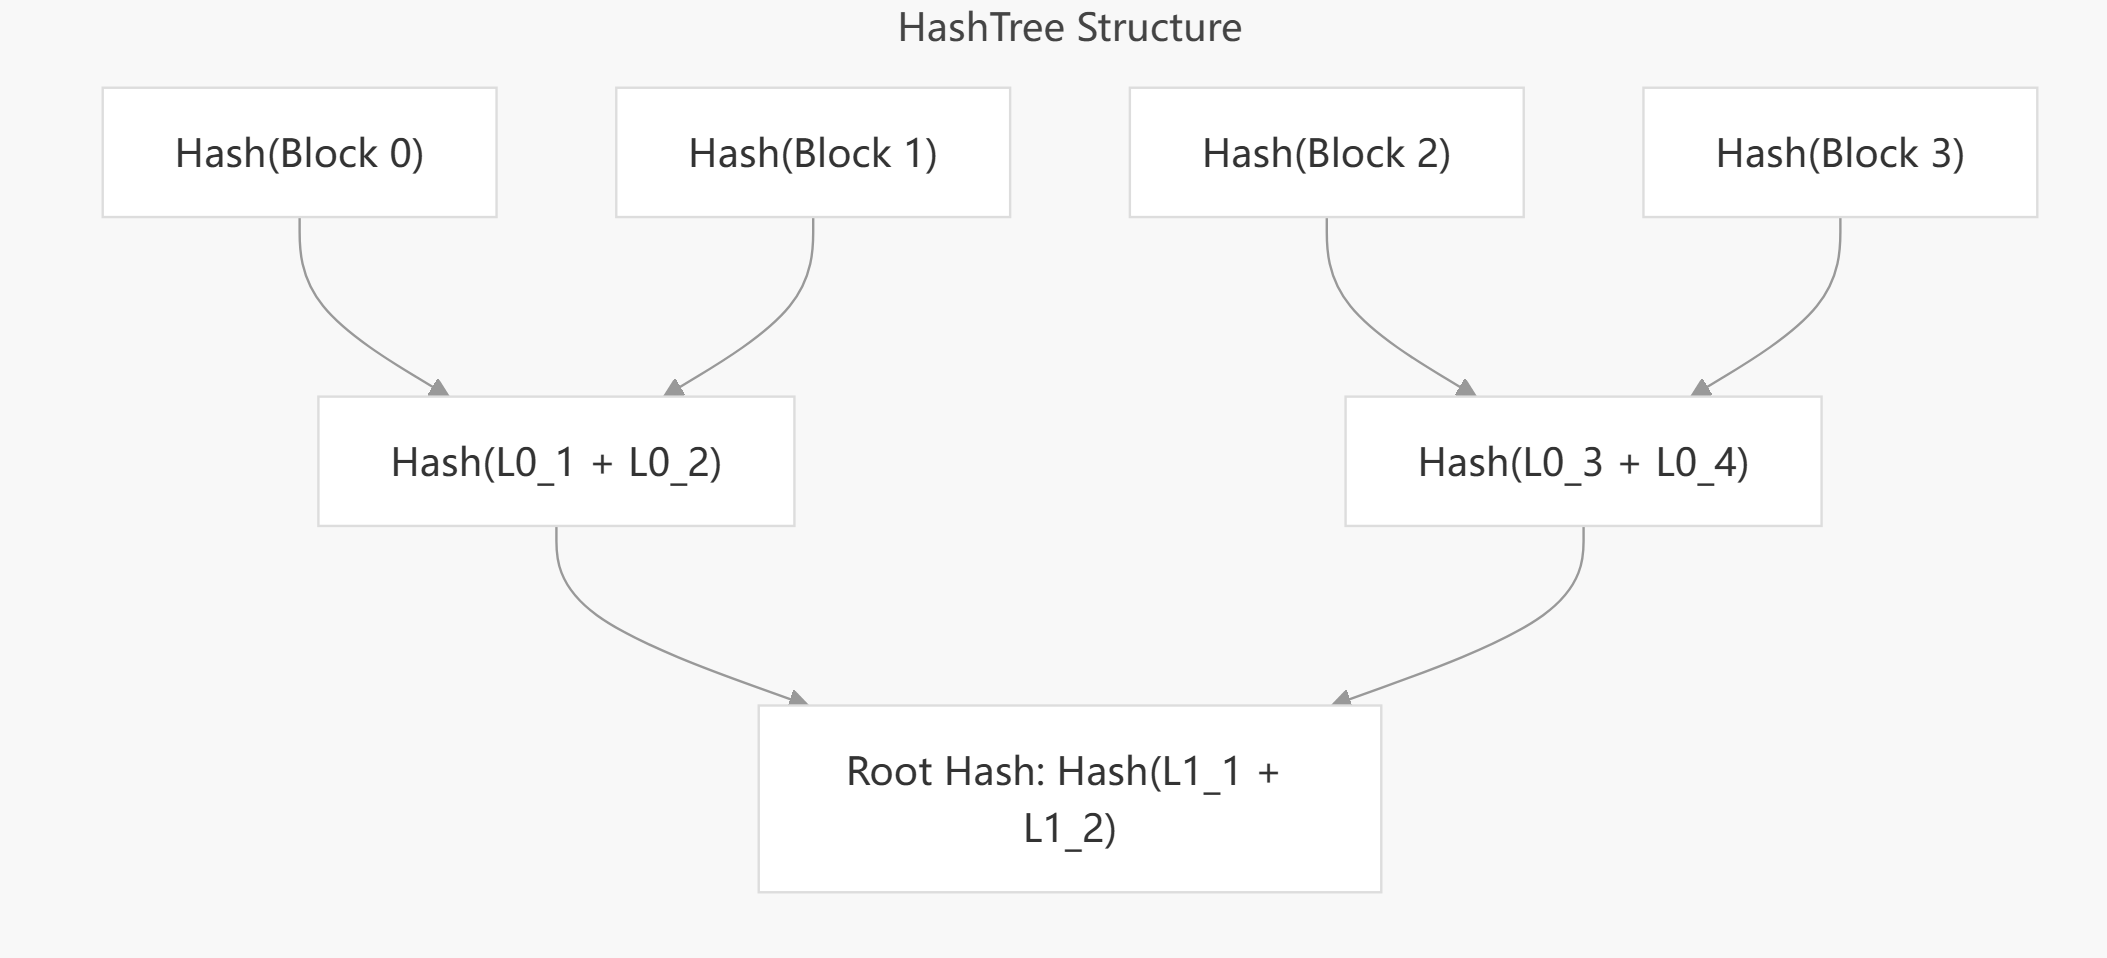
\includegraphics[width=0.9\textwidth]{merkle_tree_flow.png}
    \caption{默克尔树构建与校验数据流图}
    \label{fig:merkle_tree}
\end{figure}

\subsection{BlockDevice 抽象与可组合映射器链调研}

本项目调研并借鉴了星绽操作系统的 \texttt{BlockDevice} trait 设计，该 trait 是所有块 I/O 操作的基础接口：

\begin{lstlisting}[language=Rust, basicstyle=\ttfamily\small, breaklines=true]
pub trait BlockDevice: Send + Sync {
    fn block_size(&self) -> usize;
    fn num_blocks(&self) -> u64;
    fn read_block(&self, block_id: u64, buf: &mut [u8]) -> Result<()>;
    fn write_block(&self, block_id: u64, buf: &[u8]) -> Result<()>;
}
\end{lstlisting}

所有 I/O 方法均返回 \texttt{Result<()>}，其中错误被封装在 \texttt{DmError} 枚举中。该 trait 要求实现 \texttt{Send} 和 \texttt{Sync}，使得所有后端均可安全地跨线程共享。

基于此抽象，本项目采用类似装饰器（Decorator）的设计模式：映射器（如 \texttt{DmCryptDevice} 和 \texttt{DmVerityDevice}）既实现了 \texttt{BlockDevice} trait，又在内部包装另一个实现了 \texttt{BlockDevice} 的对象，从而支持功能的任意堆叠与组合。例如，典型的栈可以是 \texttt{FileBlockDevice $\to$ DmCryptDevice $\to$ DmVerityDevice}。

\begin{figure}[H]
    \centering
    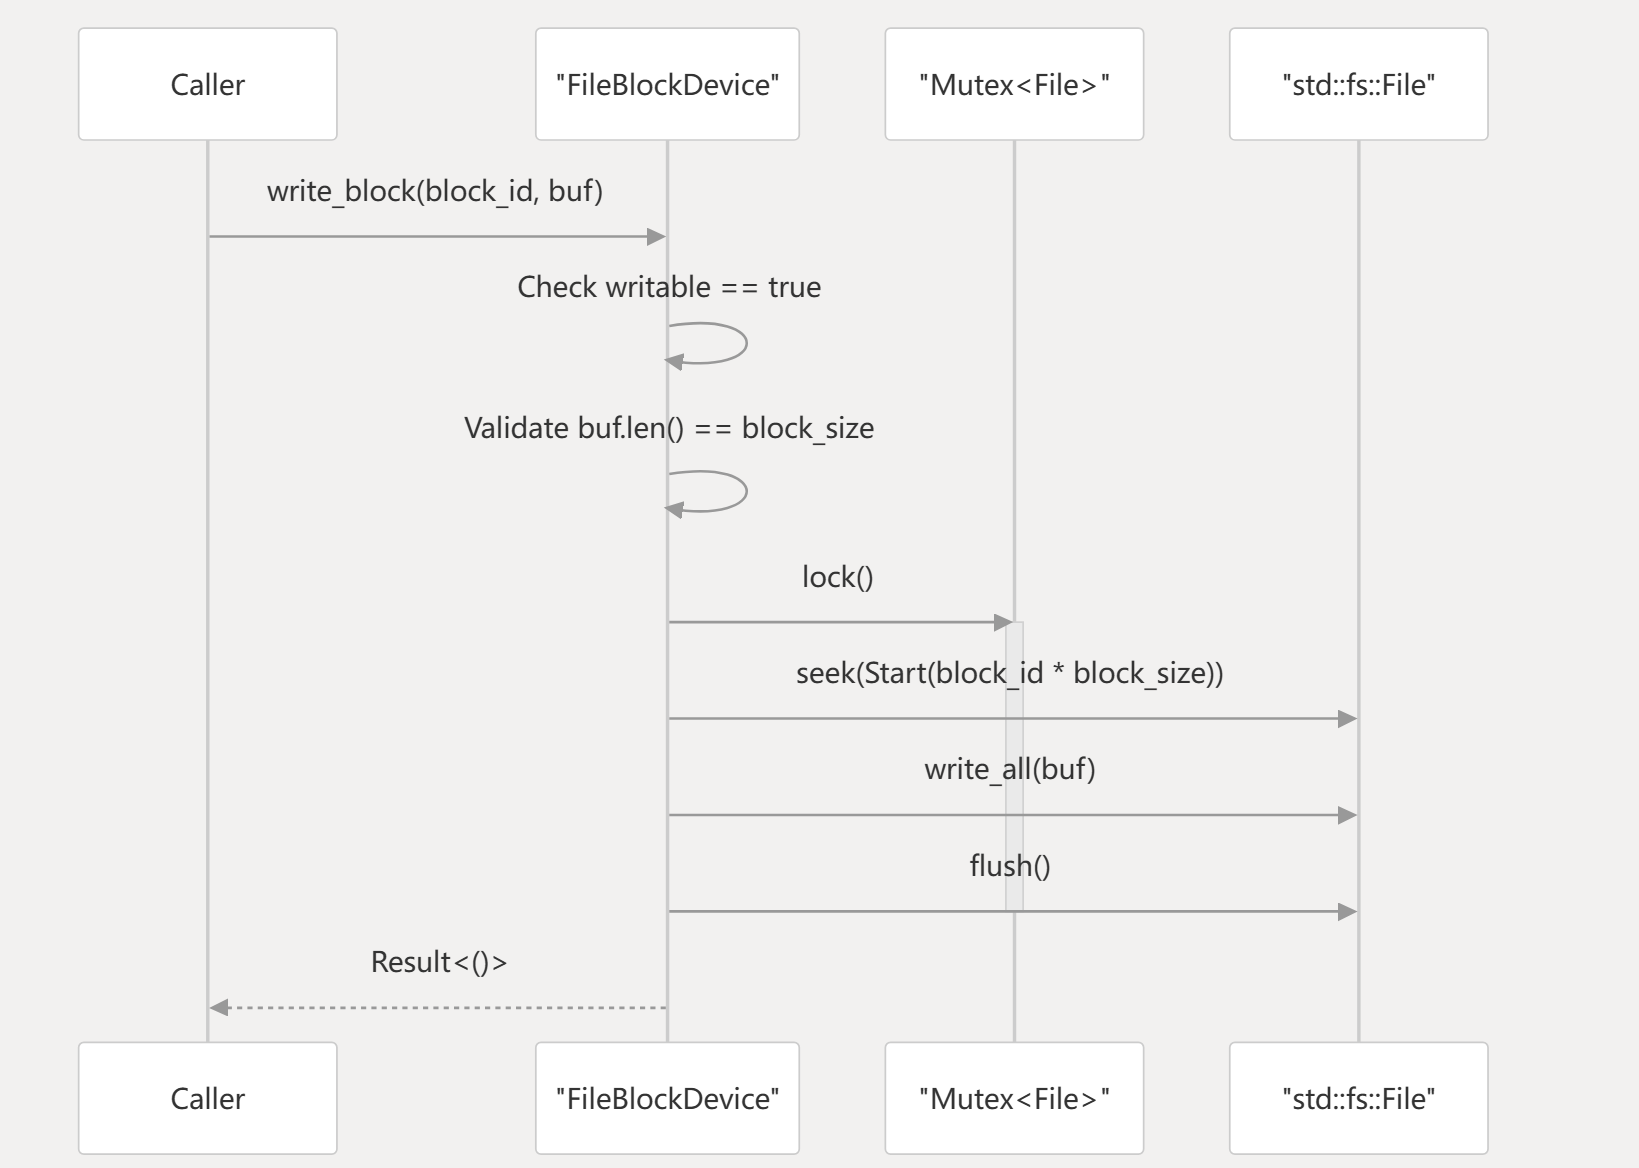
\includegraphics[width=0.9\textwidth]{blockdevice_trait_uml.png}
    \caption{BlockDevice Trait 与后端实现关系图}
    \label{fig:blockdevice_trait}
\end{figure}

该抽象已在用户态（\texttt{dmctl} 使用 \texttt{FileBlockDevice}）和星绽内核（\texttt{aster-dm} 使用 \texttt{VirtioBlkAdapter}）中得到统一实现，验证了跨环境可移植性的可行性。

\subsection{Rust 在可信存储领域的独特优势}

选择 Rust 而非 C 实现可信存储模块，具有以下独特优势：

\begin{enumerate}
    \item \textbf{内存安全}：Rust 的所有权和借用检查在编译期杜绝了悬垂指针、use-after-free 和缓冲区溢出——这些正是 C 内核中安全漏洞的主要来源（据统计约占 Linux 内核漏洞的 65\%）。在可信存储场景中，内存安全漏洞可能导致密钥泄露或完整性绕过。
    
    \item \textbf{类型系统编码安全属性}：Rust 的类型系统可以将安全属性编码到类型中。例如，本项目中的 \texttt{TargetCapabilities} 结构体使组合栈的安全能力（confidentiality、integrity、read\_only）可在编译期静态检查。
    
    \item \textbf{零成本抽象}：Rust 的 trait 和泛型不会引入运行时开销，使得抽象（如 \texttt{BlockDevice}）可以像手写 C 代码一样高效，同时保持代码可复用性。
    
    \item \texttt{Send} 和 \texttt{Sync} 的自动推导：Rust 通过这两个标记 trait 在编译期保证线程安全，避免了 C 内核中因锁使用不当导致的竞态条件。
    
    \item \textbf{更安全的错误处理}：\texttt{Result<T, E>} 强制开发者显式处理错误，避免了 C 内核中因错误码被忽略而导致的静默失败。
\end{enumerate}

本项目正是 Rust 在可信存储领域优势的实践验证——我们使用相同的核心算法（AES-XTS、SHA-256）实现了与 Linux 兼容的可信存储，同时获得了 Rust 提供的安全保障。

\subsection{参考实现与开源生态调研}

\begin{table}[H]
    \centering
    \begin{tabular}{p{0.20\textwidth}p{0.32\textwidth}p{0.38\textwidth}}
        \toprule
        \textbf{名称} & \textbf{来源/位置} & \textbf{参考内容与启示} \\
        \midrule
        Linux 内核 dm-crypt & \texttt{\seqsplit{drivers/md/dm-crypt.c}} & XTS 实现细节、plain64 IV 生成、table 格式解析 \\
        Linux 内核 dm-verity & \texttt{\seqsplit{drivers/md/dm-verity.c}} & Merkle 树 on-disk 布局、验证逻辑、缓存策略 \\
        cryptsetup 工具 & \texttt{\seqsplit{https://gitlab.com/cryptsetup/cryptsetup}} & 用户态控制协议、LUKS 格式、plain 模式 open/close \\
        RustCrypto \texttt{aes} & \texttt{\seqsplit{https://crates.io/crates/aes}} & AES 算法接口设计参考（本项目为独立实现） \\
        RustCrypto \texttt{xts-mode} & \texttt{\seqsplit{https://crates.io/crates/xts-mode}} & XTS 模式 API 参考（本项目为独立实现） \\
        NIST SP 800-38E & \texttt{\seqsplit{nvlpubs.nist.gov/nistpubs/Legacy/SP/}} & XTS-AES 模式标准定义 \\
        FIPS PUB 180-4 & \texttt{\seqsplit{nvlpubs.nist.gov/nistpubs/FIPS/}} & SHA-256 算法标准 \\
        Asterinas 源码 & \texttt{\seqsplit{https://github.com/asterinas/asterinas}} & OSTD 框架、BIO 接口、组件系统 \\
        Asterinas ATC'25 论文 & USENIX ATC 2025 & Framekernel 架构、TCB 最小化设计理念 \\
        《The Rust Programming Language》 & \texttt{\seqsplit{https://doc.rust-lang.org/book/}} & Rust 系统编程、\texttt{no\_std} 开发 \\
        \bottomrule
    \end{tabular}
\end{table}

\subsection{兼容性验证策略调研}

为确保与 Linux 生态的互操作性，本项目设计了分层兼容性验证策略：

\begin{enumerate}
    \item \textbf{算法层}：固定向量测试——AES-XTS 已知明文测试向量、SHA-256 标准测试向量（空字符串、\texttt{"abc"}）；
    \item \textbf{协议层}：与 Linux 内核 dm-crypt 逐字节比对——同一密钥（512 位）、同一明文（0x5a 填充的一个扇区）、同一扇区号（扇区 0）生成的密文 SHA-256 一致；
    \item \textbf{工具层}：在 Asterinas KVM 中运行标准 \texttt{cryptsetup} 工具（plain 模式），验证 \texttt{open}、\texttt{dd read}、\texttt{close} 完整流程（R01）；
    \item \textbf{性能层}：使用与 Linux 相同的 fio 参数和 workload，在同一 backing image 上分别测试，确保可比性；
    \item \textbf{正确性层}：通过物理篡改（单字节翻转）验证 dm-verity 的检测能力，确保完整性边界未被削弱（V03--V07）。
\end{enumerate}

\section{技术可行性评估}

基于上述调研，本项目从以下维度评估技术可行性：

\begin{table}[H]
    \centering
    \begin{tabular}{p{0.20\textwidth}p{0.35\textwidth}p{0.35\textwidth}}
        \toprule
        \textbf{维度} & \textbf{风险评估} & \textbf{应对措施} \\
        \midrule
        算法正确性 & \textbf{低风险}：AES-XTS 和 SHA-256 有明确标准和参考实现 & 固定向量测试 + Linux 逐字节比对 \\
        Linux 兼容性 & \textbf{中风险}：plain64 IV 和 XTS 实现细节易出错 & 早期编写交叉验证脚本，迭代修正 \\
        Asterinas 集成 & \textbf{中风险}：BIO 接口和启动流程需要深入理解 & 补丁序列渐进式集成，每步独立验证 \\
        性能达标 & \textbf{中风险}：虚拟机环境 I/O 性能波动大 & 固定五轮、交替顺序、保留原始数据 \\
        优化不削弱安全 & \textbf{高风险}：缓存可能绕过完整性校验 & “先认证后插入”设计原则 + 计数器验证 \\
        \bottomrule
    \end{tabular}
\end{table}

项目的总体可行性判断为\textbf{高可行}，理由如下：

\begin{enumerate}
    \item 核心算法有明确的标准（NIST、FIPS）和参考实现（Linux 内核），验证手段成熟；
    \item 双目标架构（用户态 + 内核态）使用户态可作为“安全网”，在进入内核前充分验证算法和逻辑；
    \item Asterinas 提供了清晰的组件接入接口（\texttt{Components.toml}、\texttt{aster-cmdline}、\texttt{aster-block}），集成路径明确；
    \item 性能测试合同（\texttt{benchmark\_contract.md}）固定了环境、参数、轮数和统计口径，结果可复现、可审计。
\end{enumerate}

\section{小结}

本章从赛题要求、赛题特征、技术挑战、课程关联、相关技术调研（含 Linux Device Mapper、星绽架构、AES-XTS、SHA-256、默克尔树、\texttt{BlockDevice} 抽象、Rust 优势）、参考实现和兼容性验证策略十个维度对比赛题目进行了全面分析。

核心调研结论包括：
\begin{enumerate}
    \item Linux Device Mapper 框架提供了成熟的 dm-crypt/dm-verity 参考实现，但 Asterinas 的内核接口与之不同，需要从头实现 Rust 适配层；
    \item AES-256-XTS 和 SHA-256 有明确的标准规范，通过固定向量和 Linux 逐字节比对可验证兼容性；默克尔树的 on-disk 布局设计使得标准 ext2 镜像可与哈希树共存；
    \item Rust 的所有权系统、类型系统和零成本抽象为可信存储模块提供了 C 语言无法比拟的内存安全和可组合性；\texttt{BlockDevice} trait 的统一抽象为跨环境可移植性奠定了基础；
    \item 双目标架构（用户态验证 + 内核态集成）和分层兼容性验证策略确保了项目的可验证性和可复现性；
    \item 赛题要求的 QEMU + virtio-blk 标准化测试环境已在本项目中完整实现并用于所有验证。
\end{enumerate}

基于统一抽象、渐进式集成和可观测性内置的技术路线，项目具备充分的可行性和可验证性。后续章节将详细阐述基于这些分析得出的系统架构设计。